\documentclass[12pt,a4paper]{article}
\usepackage{xeCJK}
\usepackage{fontspec}
\setmainfont{Times New Roman}
\setCJKmainfont{PingFang TC}
\usepackage[colorlinks=true, urlcolor=blue, linkcolor=red]{hyperref}
\usepackage{amsmath, amsfonts, amssymb, amsthm, algorithm, booktabs, listings}
\DeclareMathAlphabet{\mathbbold}{U}{bbold}{m}{n}
\usepackage[dvipsnames,usenames]{xcolor}
\usepackage[noend]{algpseudocode}
\usepackage{tikz}
\usepackage{fancyhdr}
\usepackage{geometry}
\newgeometry{top=2cm, bottom=2cm, left=1.5cm, right=1.5cm}
\usepackage[shortlabels]{enumitem}
\usepackage{cleveref}
\usepackage{mdframed}
\usepackage[most]{tcolorbox}
\hypersetup{citecolor=blue}
\usepackage{subcaption}
\theoremstyle{definition}
\newtheorem{definition}{Definition}[subsection]
\newtheorem{statement}{Statement}[subsection]
\newtheorem{theorem}{Theorem}
\newtheorem{lemma}[theorem]{Lemma}
\newtheorem{claim}[theorem]{Claim}
\usepackage[backend=biber,style=alphabetic,sorting=ynt]{biblatex}
\hypersetup{linkcolor=black}
\addbibresource{references.bib}
\pagestyle{fancy}

\input{shun4colors}
\newcommand{\bs}{\textbackslash}
\newcommand{\boxtxt}[1]{\boxed{\text{#1}}}
\newcommand{\op}[1]{\operatorname{#1}}
\newcommand{\OPT}{\mathrm{OPT}}

\tcbuselibrary{listings}
\newtcblisting{shuncode}[1][]{
  listing only,
  listing options={
      language=C,
      basicstyle=\ttfamily\small,
      keywordstyle=\color{blue},
      commentstyle=\color{green!50!black},
      stringstyle=\color{red}
  },
  colframe=cyan!80!black,
  colback=cyan!10,
  title={#1},
  enhanced,
}

\newtcblisting{shuncmd}[1][]{
  listing only,
  listing options={
    language=bash,
    basicstyle=\ttfamily\small,
    keywordstyle=\color{blue},
    commentstyle=\color{green!50!black},
    stringstyle=\color{red},
    breaklines=true
  },
  colframe=cyan!80!black,
  colback=cyan!10,
  title={#1},
  enhanced,
}

\newcommand{\shunsc}[1]{%
  \textsf{\textsc{#1}}
}

\newcommand{\shuncal}[1]{%
  \mathsf{\mathcal{#1}}
}

\newcommand{\hn}{
  \vspace{0.5em}
}

\newcommand{\nl}{
  \vspace{1.0em}
}

\lhead{Principles of Microeconomics}
\chead{Notes}
\rhead{Shun (@shun4midx)}

\begin{document}
\begin{center}
  {\Large \bf Principles of Microeconomics Notes}\\[8pt]
  \textbf{Author:} Shun (@shun4midx)
\end{center}

\bluesec{Chapter 1: Ten Principles of Economics}

\noindent Economists study how individual people make \textbf{decisions}, how people \textbf{interact} with one another, and the \textbf{forces and trends} that affect the economy as a whole. \\

\bluesec{How People Make Decisions}

\purplesec{Principle 1: People face trade-offs}

\pinkbox{Key Idea}{
    To get one thing we like, we must have to \textbf{give up} another --- any decision making is \textbf{trading off} one goal against another.
}

\noindent Economic examples: Taiwan's \textbf{Defense Budget Trade-Off} (Defense can go to defense vs national health insurance) \\

\pinkbox{Key Idea}{
    One main trade-off society faces is: \textbf{Efficiency vs Equality}
}

\noindent Economic example: Policies that \hl{redistribute income from the rich to the poor} may increase equality, but decrease efficiency due to the decreased reward for working hard. \\

\purplesec{Principle 2: The cost of something is what you give up to get it}

\pinkbox{Key Idea}{
    There is always \textbf{opportunity cost}
}

\noindent Economic example: Opportunity cost of \hlbf{military service} (Conscript pay < civilian job pay, so the opportunity cost is how much one would be ``losing'' from being conscripted) \\

\purplesec{Principle 3: Rational people think at the margin}

\pinkbox{Key Idea}{
    \textbf{Marginal cost and benefit} is what is considered when we make decisions, i.e. \textbf{marginal thinking}
}

\noindent Economic examples:
\hn\begin{itemize}
    \item The \hlbf{Water--Diamond Paradox} (water is essential, but its plentiful; diamonds are rare, so there's huge marginal benefit) $\Rightarrow$ actually led to Taiwan running short of water because of TSMC requiring a lot of water supplies, cutting irrigation to farmland (water stopped being plentiful, so its marginal value rose)
    \item Planes offering a standby seat for far less (marginal cost for one more passenger is tiny if the plane will fly anyway)
    \item \hlbf{Netflix} can set the marginal cost of watching one more movie to zero (once the monthly fee is paid, watching another film costs almost nothing extra)
\end{itemize}

\purplesec{Principle 4: People respond to incentives}

\pinkbox{Key Idea}{
    Rational people make decisions by weighing costs and benefits, so they must respond when \textbf{costs and benefits change}, mainly in the form of \textbf{incentives}
}

\noindent Economic examples:
\hn\begin{itemize}
    \item \hlbf{Taipei's Trash Policy (Succeeding)}: Households must use the official garbage bag, so \textbf{every extra bag now has a real marginal cost}
    \item \hlbf{Seat Belt Law (Backfiring)}: Seat belts made accidents less costly by reducing risk of injury, which decreased the benefit of driving safely; due to time and effort taken to drive safely, people drived less safely
\end{itemize}

\bluesec{How People Interact}

\purplesec{Principle 5: Trade can make everyone better off}

\pinkbox{Key Idea}{Trading with others lets each person \textbf{specialize in what they do best}, so everyone can buy a greater variety of goods and services at a lower cost than they could achieve alone}

\noindent Economic example: \hl{Taiwan trading chips for oil, coal, and natural gas} \\

\purplesec{Principle 6: Markets are usually a good way to organize economic activity}

\pinkbox{Key Idea}{
    \textbf{Market economies} are more effective than centrally planned economies which lack the information to decide what and how to produce, and for who
}

\noindent Economic example: \hl{Taiwan's high density of convenience stores} (No planning agency decided how many stores each neighborhood needed, each store's owner just responded to the people) \\

\pinkbox{Adam Smith's Invisible Hand}{
    \textbf{Adam Smith's Invisible Hand} steers markets and households towards outcomes that maximize the well-being of society as a whole
}

\purplesec{Principle 7: Governments can sometimes improve market outcomes}

\pinkbox{Key Idea}{
    \textbf{The invisible hand} can only work if the government \textbf{enforces the rules} a market economy depends on
}

\noindent Without secure property rights, people stop producing:
\hn\begin{itemize}
    \item A farmer won't grow food if they expect the crop to be stolen before harvest
    \item A film studio won't produce movies if it cannot stop people form copying them for free
\end{itemize}

\noindent However, the invisible hand can still \textbf{fail}, likely from two common sources:
\begin{itemize}
    \item \textbf{Externality}: The effect of one person's actions on a bystander (e.g. pollution)
    \item \textbf{Market power}: A single actor's ability to influence market prices (e.g. monopoly)
\end{itemize}

\noindent Economic example: \hlbf{Taiwan's National Health Insurance (Successful)}
\begin{itemize}
    \item A private health insurance market tends to fail (insurers want to avoid the sickest customers; healthy people are tempted to skip coverage until they need it)
    \item Taiwan's NHI program making \textbf{enrollment mandatory for essentially everyone} corrects a market failure (prevents the market from unraveling) and also promotes \textbf{equality}
\end{itemize}

\bluesec{How the Economy as a Whole Works}

\purplesec{Principle 8: A country's standard of living depends on its ability to produce goods and services}

\pinkbox{Key Idea}{
    Raising productivity leads to raising living standards
}

\noindent Economic example: \hlbf{The Taiwan Miracle} (mostly agricultural economy to an advanced semiconductor production) \\

\purplesec{Principle 9: Prices rise when the government prints too much money}

\pinkbox{Key Idea}{
    In almost any case of high or persistent \textbf{inflation}, the underlying cause is likely that the \textbf{government created money faster} than the \textbf{economy producing goods and services}
}

\purplesec{Principle 10: Society faces a short-run trade-off between inflation and unemployment}

\pinkbox{Key Idea}{
    Increasing the amount of money in the economy stimulates spending, which encourages companies to hire more and thus lower unemployment. However, this may drive to inflation. >\_<
}

\newpage

\bluesec{Chapter 2: Thinking Like an Economist}

\purplesec{The Economist as a Scientist}

\pinkbox{Key Idea}{
    Economists can rely on \textbf{natural experiments} to better understand the economy
}

\noindent Economic examples: War and the Price of Oil (US-Israel war against Iran), COVID-19 (comparing regions that locked down hard vs regions that did not) \\

\purplesec{The Circular-Flow Diagram}

\noindent The diagram simplifes the economy down to two decision makers---firms and households---interacting in two markets. It leaves out government and international trade

\begin{figure}[h]
    \centering
    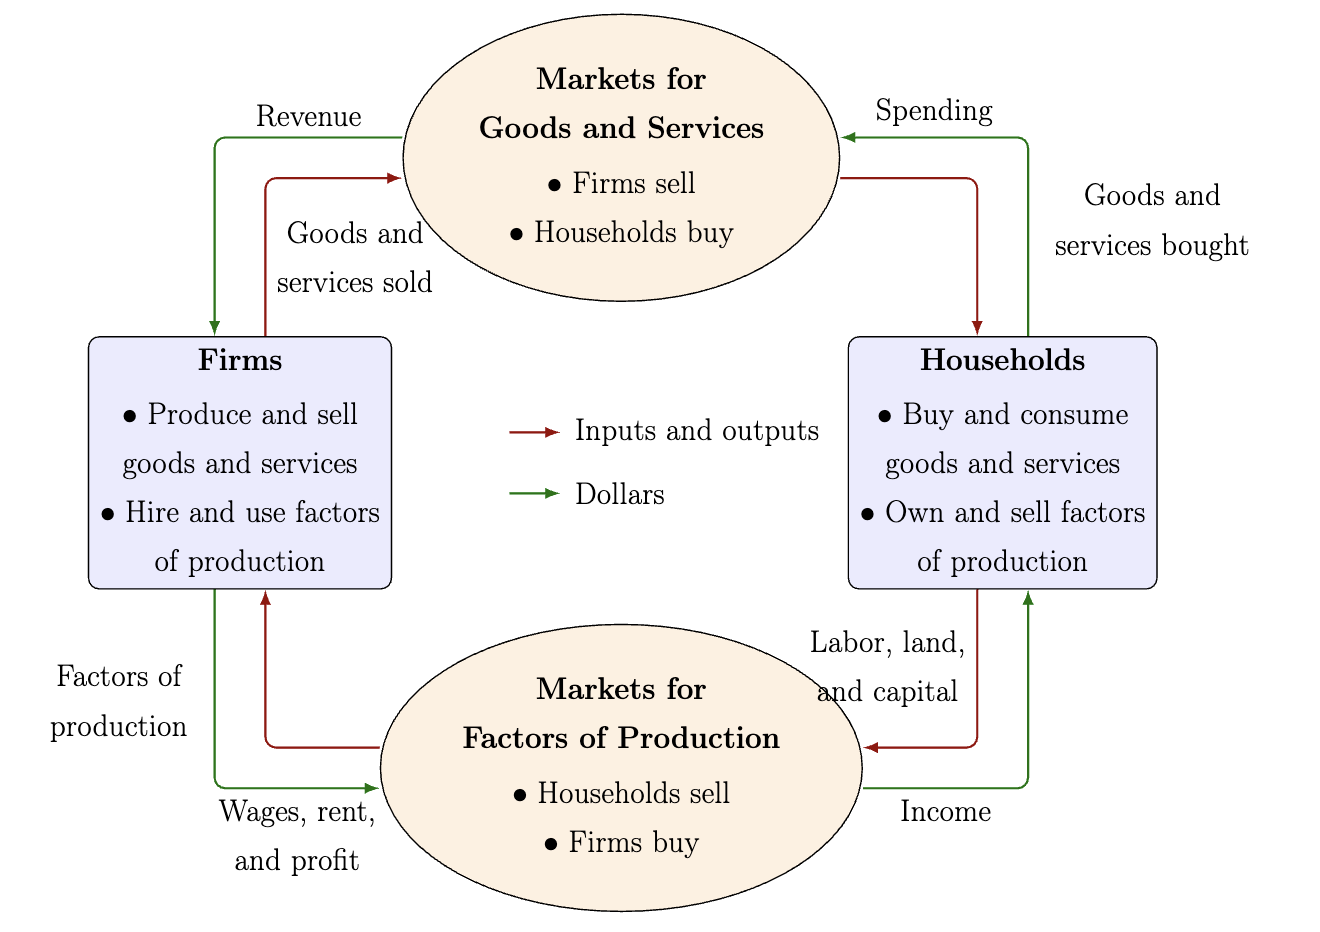
\includegraphics[width=0.85\textwidth]{imgs/circular_flow_diagram.png}
    \caption{The circular-flow diagram}
    \label{fig:circular_flow_diagram}
\end{figure}

\purplesec{The Production Possibilities Frontier (PPF)}

\noindent We can categorize an economy into one of three categories:

\hn\begin{itemize}
    \item \hlbf{Efficient}: Sit \textbf{on} the frontier
    \item \hlbf{Infeasible}: Lie \textbf{outside} the frontier --- unachievable
    \item \hlbf{Inefficient}: Lie \textbf{inside} the frontier --- some resources are unused
\end{itemize}

\noindent \hlbf{Economic growth} shifts the frontier, as shown below:
\begin{figure}[h]
    \centering
    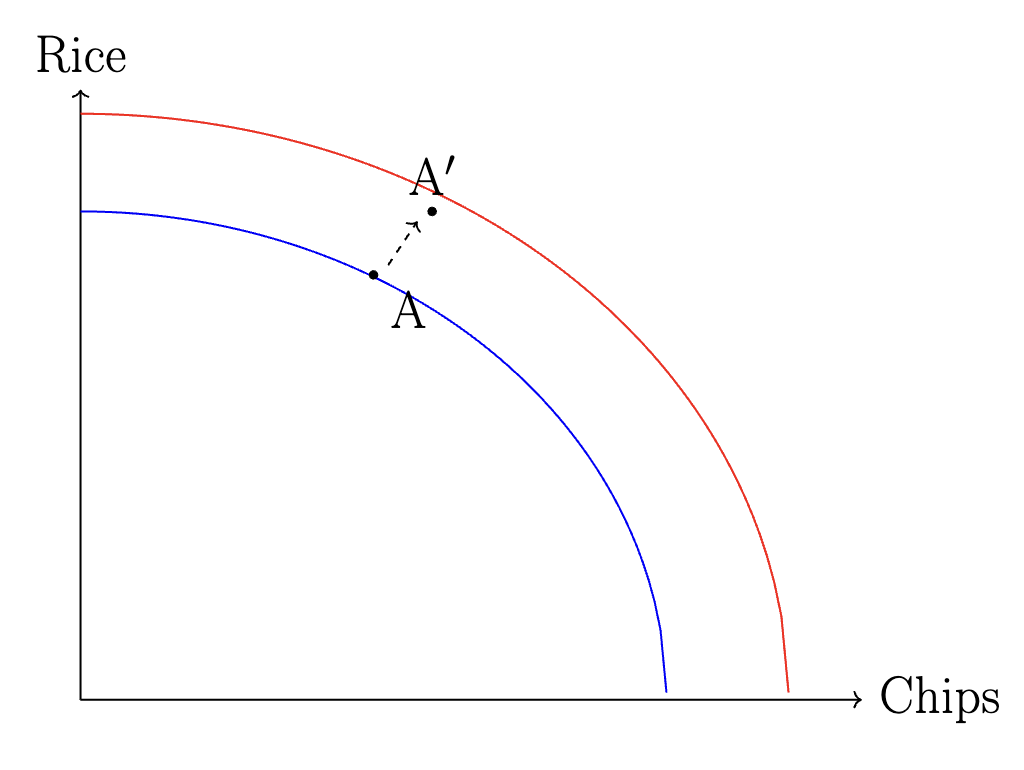
\includegraphics[width=0.5\textwidth]{imgs/econ_growth_frontier.png}
    \caption{Economic growth shifting the frontier}
    \label{fig:econ_growth_frontier}
\end{figure}

\purplesec{The Economist as Policy Adviser}

\pinkbox{Key Idea}{
    When economists explain the effects of a policy, they act as scientists and are objective. When they \textbf{recommend} a policy, they act as \textbf{policy advisers}, which are subjective.
}

\purplesec{Positive vs Normative Statements}
\pinkbox{Key Idea}{
    Economists may \textbf{disagree} about \textbf{competing positive theories}; they may disagree about \textbf{normative statements} since they \textbf{hold different values}.
}

\newpage

\bluesec{Chapter 3: Interdependence and the Gains from Trade}

\purplesec{Main Example}

\pinkbox{Setting}{
    There are \textbf{two countries} (Taiwan and Cambodia), each only produce \textbf{two goods} (chip batches and tons of rice), using only one input (labor). We also assume each country switches between two goods at a constant rate, and works for \textbf{8 hours a day}. The labor conditions are given below.
}

\begin{table}[h]
    \centering
    \begin{tabular}{ | c c c | } 
    \hline
    & \textbf{Mins per chip batch} & \textbf{Mins per ton of rice} \\
    \hline
    Taiwan & 20 & 10 \\
    Cambodia & 60 & 15 \\
    \hline
    \end{tabular}
\end{table}

\noindent We see, if each country spends 4 hours on each good each day, Taiwan can produce \textbf{12 batches of chips} and \textbf{24 tons of rice} a day, whereas Cambodia can produce \textbf{4 batches of chips} and \textbf{16 batches of rice} a day. Although any other point on the PPF is possible. Clearly, \hl{Taiwan has an \textbf{absolute advantage}}. \\

\begin{figure}[h]
    \centering
    \begin{minipage}{0.48\textwidth}
        \centering
        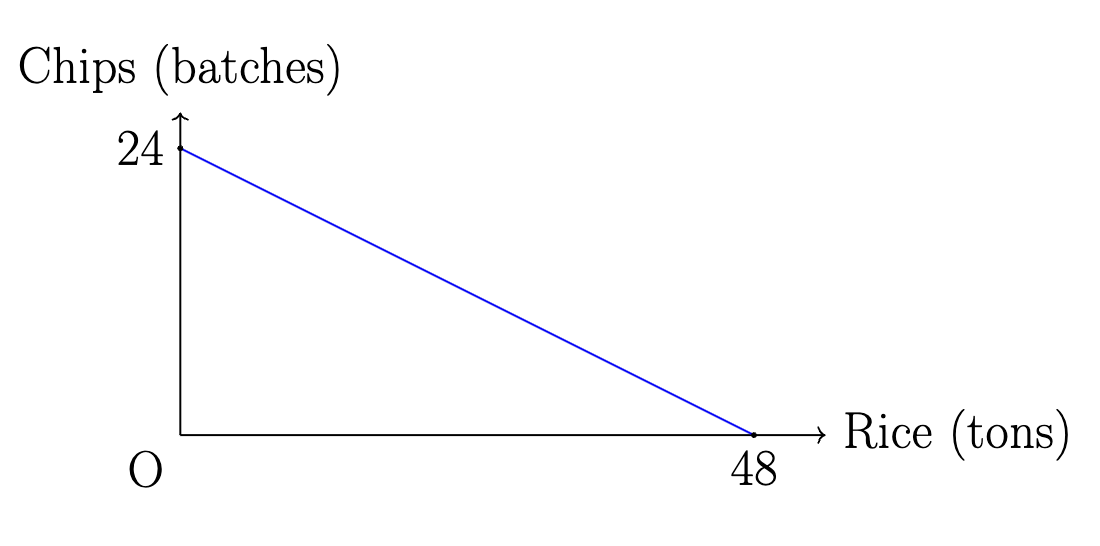
\includegraphics[width=\textwidth]{imgs/ch03_tw_ppf.png}
        \caption{Taiwan's PPF}
        \label{fig:ch03_tw_ppf}
    \end{minipage}
    \hfill
    \begin{minipage}{0.48\textwidth}
        \centering
        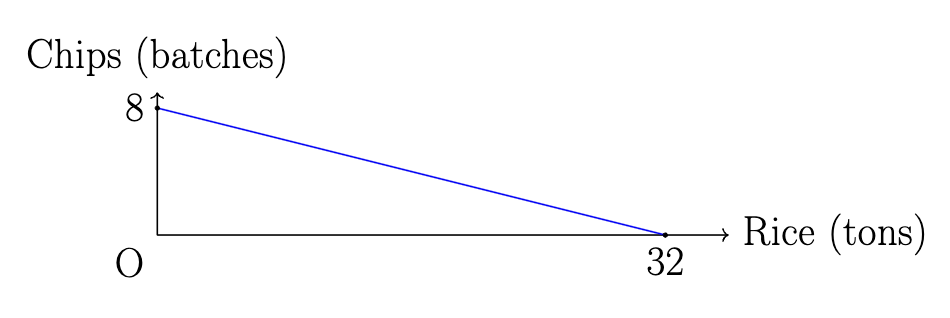
\includegraphics[width=\textwidth]{imgs/ch03_cam_ppf.png}
        \caption{Cambodia's PPF}
        \label{fig:ch03_cam_ppf}
    \end{minipage}
\end{figure}

\noindent However, in terms of \hlbf{opportunity cost}, we see

\begin{table}[h]
    \centering
    \begin{tabular}{ | c c c | } 
    \hline
    & \textbf{Opportunity cost of 1 chip batch} & \textbf{Opportunity cost of 1 ton of rice rice} \\
    \hline
    Taiwan & 2 tons of rice & 0.5 chip batches \\
    Cambodia & 4 tons of rice & 0.25 chip batches \\
    \hline
    \end{tabular}
\end{table}

\noindent Then, Taiwan has a comparative advantage in chips (2 < 4) and Cambodia has a comparative advantage in rice (0.25 < 0.5). \\

\noindent Suppose Taiwan shifts more time towards chips, producing \textbf{18 chip batches and 12 tons of rice} a day, and Cambodia specializes completely in rice, producing \textbf{32 tons of rice and no chips}. \\

\noindent Suppose Cambodia trades 15 tons of rice to Taiwan in exchange for 5 chip baches (3 tons of rice per chip batch). This lies in \textbf{between Taiwan's opportunity cost of a chip batch (2 tons of rice) and Cambodia's (4 tons of rice)}, which is \textbf{exactly the range} which both countries are willing to trade. \\

\noindent Notice, after trading, both countries get to be above their PPFs, which is a \textcolor{blue}{gain for both sides}.

\begin{figure}
    \centering
    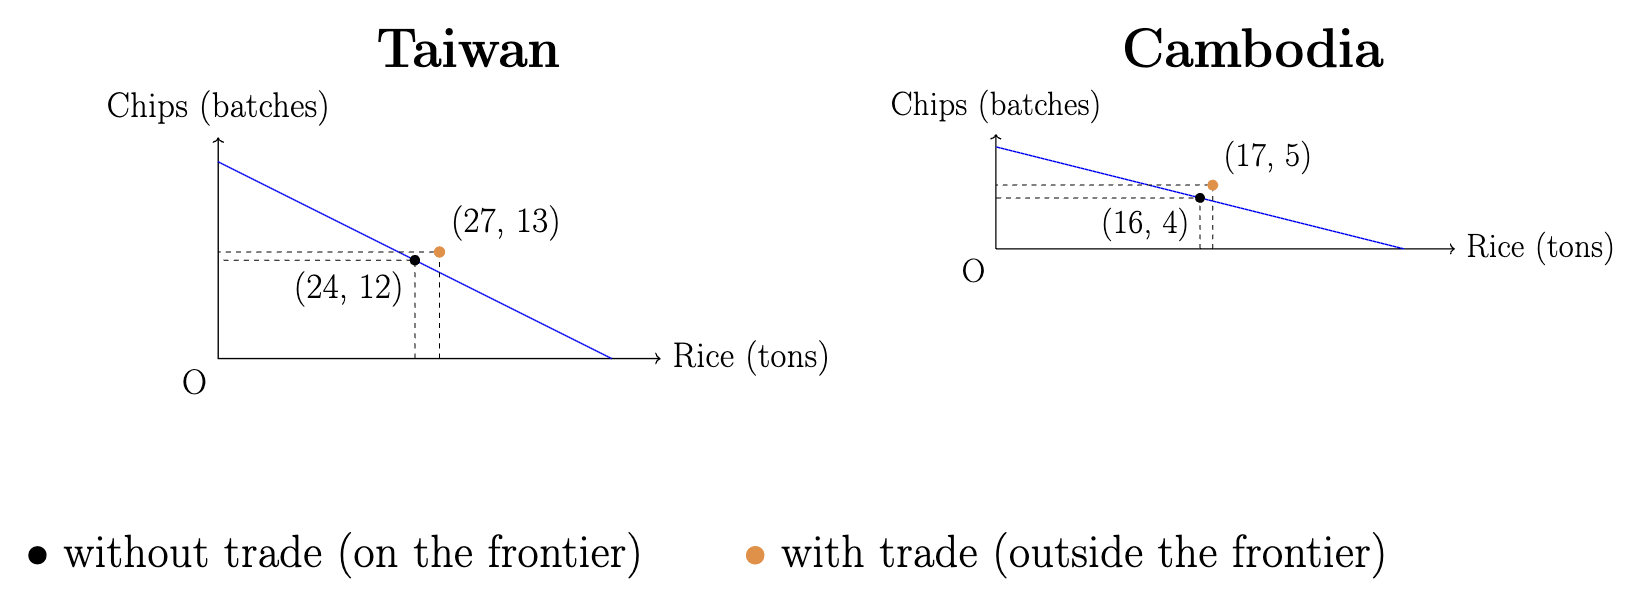
\includegraphics[width=0.95\textwidth]{imgs/ch03_tw_cam_ppf.png}
    \caption{Taiwan and Cambodia's PPF vs after trading}
    \label{fig:ch03_tw_cam_ppf}
\end{figure}

\purplesec{Other Examples}

\begin{itemize}
    \item The surgeon and her assistant: A surgeon who can type faster than anyone else in her office should still hire an assistant to handle her scheduling and paperwork, since every hour she spends on typing is an hour she is not spending on surgery (i.e. opportunity cost of an hour of typing is far higher than her assistant's)
    \item Taiwan's Rice Import Quota: It raises the country's total economic pie to import rice, but it \textbf{can hurt specific producers} (i.e. domestic rice farmers) $\Rightarrow$ \hlbf{Sometimes it's important to protect local} \\ \hlbf{producers, rather than maximizing purely for consumer benefit}
\end{itemize}

\newpage

\bluesec{[INCOMPLETE] Chapter 4: Market Forces of Supply and Demand}

\purplesec{Demand}

\noindent The demand curve slopes downward, because other things equal, a lower price means a greater quantity demanded. The demand curve shows how price affects quantity demanded, holding constant everything else that affects buyers. \hn

\begin{itemize}
    \item A \textbf{change in price} moves us along a \textbf{fixed demand curve}
    \item A change in anything else that affects demand, income, the price of related goods, tastes, expectations, or the number of buyers, \textbf{shifts the entire curve} to a new position
\end{itemize}

\pinkbox{What shifts the demand curve?}{
    \begin{itemize}
        \item \hlbf{Income}: For a \emph{normal good}, higher income raises demand (e.g. diamonds); for an \emph{inferior good}, higher income lowers demand (e.g. instant ramen)
        \item \hlbf{Prices of related goods}: A higher price of a \textbf{substitute} (e.g. coffee, for bubble tea) raises demand; a higher price for a \textbf{complement} (e.g. tapioca pearls, for bubble tea shops' costs) lowers demand for the other good
        \item \hlbf{Tastes}: Anything that makes a good more or less appealing shifts demand in the same direction
        \item \hlbf{Expectations}: Expecting \textbf{higher prices or higher income in the future} can raise demand today
        \item \hlbf{Number of buyers}: More buyers in the market raises demand at every price
    \end{itemize}
}

\end{document}